
\begin{figure}[H]
	\centering
	\begin{minipage}[b]{0.45\textwidth}
		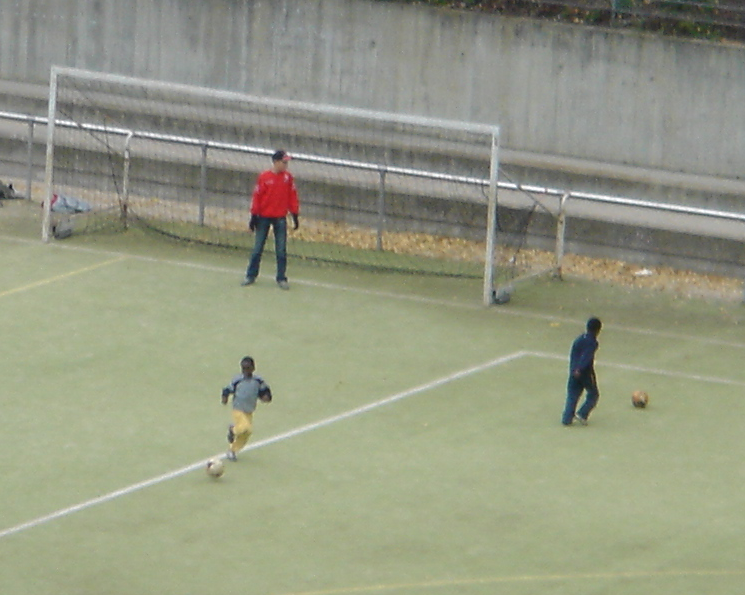
\includegraphics[width=\textwidth]{Bilder/hog1crop.png}
		\caption{(a)}
	\end{minipage}
	\hfill
	\begin{minipage}[b]{0.45\textwidth}
		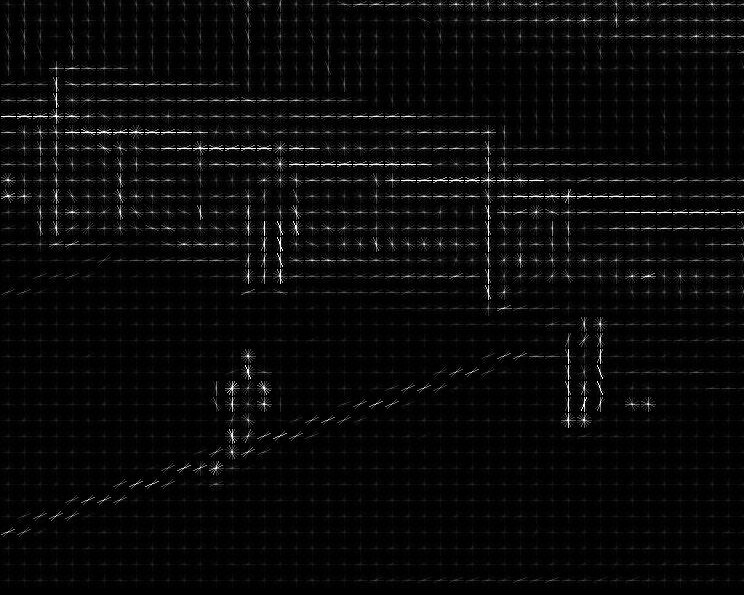
\includegraphics[width=\textwidth]{Bilder/hog2crop.jpg}
		\caption{(b)}
	\end{minipage}
	\caption{(a) Foto von drei spielenden Personen \cite{inria1}. (b) Darstellung der Gradienten, die durch einen HoG erzeugt worden sind. Die Analyse erfolgte mit Bild (a) \cite{inria1}.}
	\label{fiq: hog}
\end{figure}